\section{Entwurf}\label{entwurf}

Im folgenden sollen die aus der Analysephase  ausgearbeiteten Anforderungen zu einem Entwurf zusammen gefasst werden, in dem die notwendigen Komponenten und deren Schnittstellen genauer beschrieben werden. Zunächst soll aber das Datenmodel für die Kompetenzen und dessen Format gewählt werden.

\subsection{Format/Kompotenzmodell}

Wie in Kapitel 1 beschrieben, gibt es unterschiedliche Ansätze und widersprüchliche Meinungen um ein Modell für Kompetenzen zu beschreiben. Für den Entwurf des Empfehlungssystems sollen zunächst einige in Frage kommenden Modelle evaluiert werden. 

\subsubsection{ESCO als RDF}

ESCO wird als RDF Graph im SKOS Format zum Download angeboten. Das Vokabular\cite{esco_ontology} für dieses Schema beinhaltet unter anderem folgende relevante Klassen: 
\vspace{1em}
ESCO concepts \newline

Relationship

IRI: http://data.europa.eu/esco/modelRelationship

Beziehung zwischen zwei ESCO Säulen z.B. Occupation und Qualification.\newline

Qualification 

IRI: http://data.europa.eu/esco/modelQualification

Ein offiziell, oder formelles Zertifikat eines, oder mehrerer Kompetenzen oder Fertigkeiten. Kann verknüpft mit Skills oder Berufen sein.\newline

Skill 

IRI: http://data.europa.eu/esco/modelSkill

In dieser Klasse werden Konzepte für Fertigkeiten und Kompetenzen und Wissen zusammengefasst.\newline

 ESCO wendet hier dieselben Definitionen für diese Begriffe an, wie sie der EQF vorgibt.\cite{https://ec.europa.eu/esco/portal/escopedia/Competence}
ESCO unterscheidet in seinem Modell nicht zwischen Fertigkeiten und Kompetenzen sondern nur zwischen Fertigkeiten und Wissen. Dieser Unterschied wird durch hierarchische Strukturen implementiert.  
\newline

Occupation 

IRI: http://data.europa.eu/esco/modelOccupation

In dieser Klasse werden Berufsgruppen zusammengefasst.

\vspace{1em}

Kritik für das ESCO Modell kommt hingegen vom Bundes Ministerium für Berufliche Bildung. Es sieht mögliche negative Rückwirkungen auf duale Berufsbildungsysteme, beim Einsatz von europaweiten Teilkompetenzen und fordert eine genauere Überprüfung der Kompatibilität von ESCO mit Standards wie EQR und NQR hinsichtlich der Qualifikationsniveaus der Beschreibungen. 

\subsubsection{inLOC}

Das Projekt InLOC ermöglicht das Abbilden von mehreren Kompetenzrahmen in einem einheitlichen maschienenlesbaren Format(RDF,XML,JSON-LD). 
Auf der Projekt Website wird anhand einer exemplarischen Kompetenz des e-CF in Version 2.0 die Struktur des inLOC Informations Modells beschrieben. \newline

Das folgende Digramm zeigt die Struktur für Kompetenzen aus dem e-CF.
 Deutlich zu erkennen sind die 4 Dimensionen \textit{Kompetenzfelder, Kompetenzen, Kompetenzniveaus, Beispiele für Wissen und Fähigkeiten}
 
 \begin{figure}[htb]
 \centering
 \includegraphics[width=0.7\textwidth,angle=0]{abb/e-CF}
 \caption[Beschreibung]{e-Kompetenz in inLOC}
\label{fig:e-Kompetenz in inLOC}
\end{figure}

 
 \subsubsection{Fazit: Auswahl eines Models}
 
  Das inLOC Model findet aktuell keine Anwendung, und man müsste eine erst eine Reihe von Beispiel Daten erstellen, z.B. durch manuelles eintragen der Kompetenzen aus dem e-CF. \newline
 
 Für die Implementierung soll zunächst nur das Modell, welches durch den ESCO Katalog angeboten wird, verwendet werden. Zum einen Steht dieser Katalog in der aktuellen Version mit ca. 13.500 Einträgen zu Wissens und Fertigkeiten/Kompetenz Konzepten zum Download zur Verfügung, und ist darüber hinaus EU Länder übergreifend, was ihn für einen breiteres Spektrum an Anwendungen interessant macht. 
 Der Aspekt der Kompatibilität mit einzelnen nationalen Bildungssystemen kann vernachlässigt werden, da es nicht um die Findung einer Lösung geht, welche den Arbeitsmarkt und die Berufsbildung in gleichem Maße berücksichtigt, sondern den rein technischen Ansatz, für ein Verfahren Kompetenzen aufgrund ihrer strukturellen Modellierung zu vergleichen. 
 


\subsubsection{Datenbank}

Nachdem nun das Datenmodell für die Speicherung der Kompetenzen gewählt wurde, muss eine geeignete Datenbank gewählt werden. Das SKOS Schema des ESCO Katalogs liegt zwar bereits als gerichteter Graph, nämlich im RDF Format vor, soll aber aus Gründen der Flexibilität und Möglichkeiten in ein Datenbankmanagement System überführt werden.
Alternativ könnte mit Hilfe von SPARQL, einer graphen basierten Abfragesprache, direkt auf dem RDF Graphen gearbeitet werden 
,hier sollen jedoch von den Vorteilen eines \textit{Label Property Graphen}  Gebrauch gemacht werden. Möchte man eine Kompetenz in RDF modellieren, so muss zunächst ein Knoten für die Kompetenz selbst angelegt werden. Soll die Kompetenz neben dem \textit{Identifier} auch noch ein Namens- oder Sprachattribut hinzufügen, müssen zunächst Knoten und Beziehungen für jedes Attribut angelegt werden. Daraus resultiert ein stärkere Vernetzung des Graphen. Im \textit{LPG} können die Attribute einfach dem Kompetenzknoten hinzugefügt werden. Emil Eifrem, CEO der Open-Source Graphendatenbank \cite{Neo4j} übt Kritik an der RDF Community. So bemängelt er, dass zu wenig Rücksicht auf Entwickler und die Integration in Software Systeme genommen wird. \cite{anadiotis_2017} \newline

"There is a pool of super smart people in the Semantic Web community, but their approach is typically extremely academic. "
Warum keine RDF Technologie?

\subsection{Datenmodell}

Da der ESCO Katalog als Ontologie implementiert und im Linked Data Format als SKOS veröffentlich wird, liegen die Konzepte von Kompetenzen als hierarchische Struktur vor. Dabei gibt es ausgehend vom Root Knoten einen Unterknoten für die \textit{Kompetenzen/Fertigkeiten} Säule, von dem ausgehend sich der Baum aufspaltet in Job-spezifische und Transversale Skills. Hierarchien in SKOS werden über \textit{broader-narrower} Beziehungen hergestellt. Kompetenzen sind Teil der Konzept Klasse \textit{Skill} und werden mit der \textit{LeafGroup} und \textit{Member} Konzept Klasse strukturiert. Beispielsweise ist die Kompetenz \textit{Windows XP} Teil der Gruppe \textit{Computing} die wiederum Teil der Gruppe \textit{Job-specific skills/competences} Gruppe ist.

\begin{figure}[htb]
 \centering
 \includegraphics[width=0.7\textwidth,angle=0]{abb/graph}
 \caption[Beschreibung]{Hierarischie Struktur von Kompetenzen}
\label{fig:Beschreibung}
\end{figure}

\subsubsection{API}

 Die Funktionsweise der Recommendation Engine soll sich lediglich auf folgende Prozesse beschränken:\newline
 
 Eingabe und Ausgabe einer Kompetenz
Berechnung von Ähnlichkeiten im Graphen durch Graph Traversierung und Abfragen an die Datenbank. Über das HTTP Protokoll sollen Anwendungen mit dem Empfehlungsdienst kommunizieren können. Dabei werden die CRUD Methoden POST und GET auf entsprechenden Endpunkten aufgerufen. 
\newline

Die Zweite Komponente muss eine Datenbankanbindung für die Datenbank gewährleisten, und Daten aus der Eingabe in Anfragen an die Datenbank verarbeiten, sowie Ergebnisse der Anfragen zurückliefern. Falls die Anfragensprache der Datenbank nicht alle Möglichkeiten ausschöpfen kann die Ergebnisse wie gewünscht zu filtern, können in der zweiten Komponente weitere Algorithmen implementiert werden.\newline

Die Anwendung ist also wenig Komplex. Ein viel höherer Implementierungsaufwand ist den Vergleichsalgorithmen, bzw Graph Queries zuzurechnen. 

\begin{figure}[htb]
 \centering
 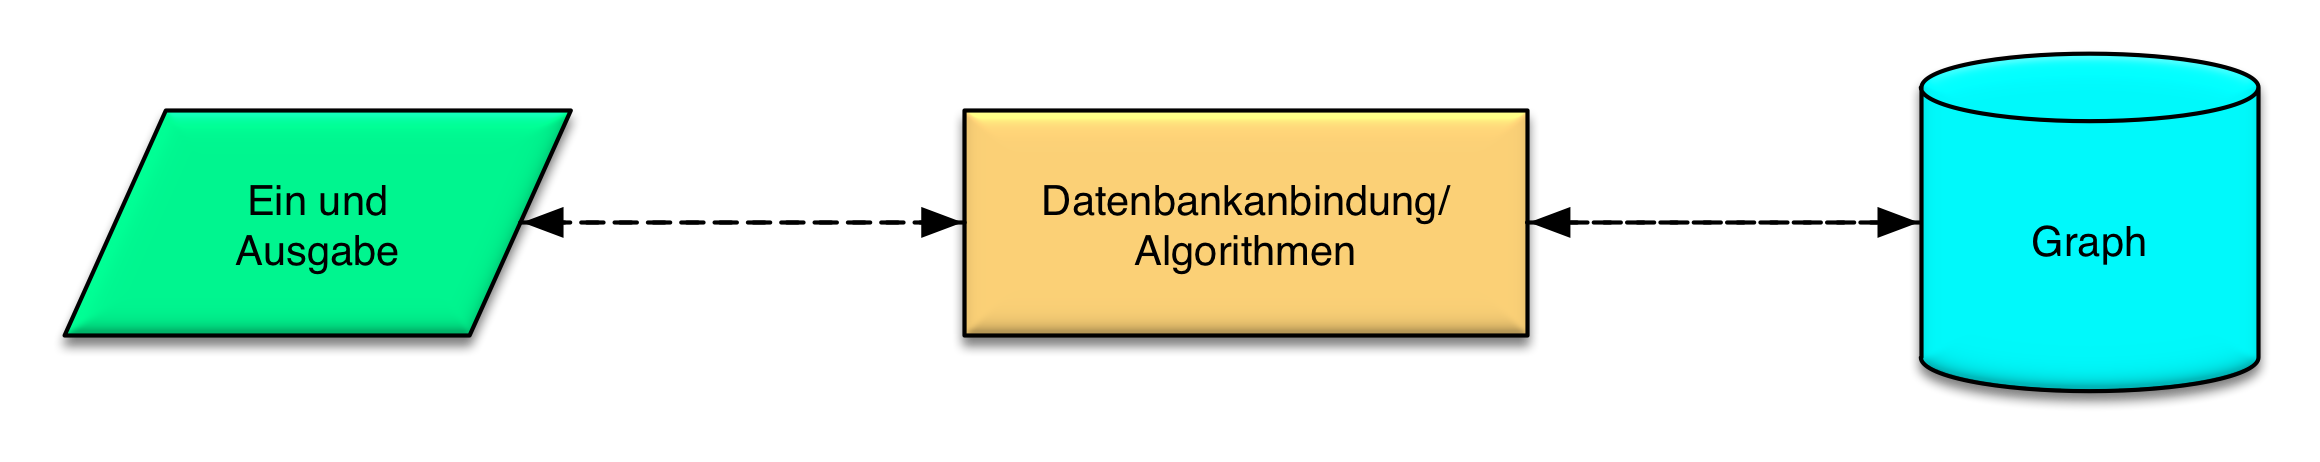
\includegraphics[width=0.7\textwidth,angle=0]{abb/entwurf}
 \caption[Beschreibung]{Entwurf}
\label{fig:Entwurf}
\end{figure}



\subsection{Anfragen Formulieren}

Bevor Abfragen in einer Abfragensprache für die Datenbank erstellt werden, sollen diese zunächst in natürlicher Sprache formuliert werden, und später in eine entsprechende Abfragensprache  transformiert werden. Dabei soll das zuvor erstellte  Datenmodell helfen. Anhand der Knoten und Kanten können die Entitäten und deren Beziehungen identifiziert werden, aus diesen lassen sich dann Abfrage Sätze formulieren. In der Formulierung wird zum Ausdruck gebracht, welche die gewünschten Knoten sind und welcher Bedingung das Ergebnis unterliegt. Die Einfachste Abfrage würde demnach lauten: \textit{Zeige Alle Knoten}. Das Ergebnis wäre der Komplette Graph. Eine spezifischeres Ergebnis erhält man durch das hinzufügen von Bedingungen. \newline \textit{  Zeige Alle Knoten, mit dem Attribut {name = \textbf{\texttt{\string{Softwareentwicklung\string}}}}}. 


